%!TEX encoding = UTF-8 Unicode
%!TEX program = xelatex
%!TEX TS-program = xelatex
%%
%-------------------------------------------------------------%
% A LaTeX template for slides in Chinese
% Author: Yuxuan Li (李宇轩)
% School of Information Science and Engineerning
% Southeast University
% Nanjing, China
% April, 2020
% Version 1.0
%-------------------------------------------------------------%

\documentclass{beamer}
\usefonttheme[onlymath]{serif}
% See https://hartwork.org/beamer-theme-matrix/ for more themes
\usetheme{Madrid}
\setbeamertemplate{theorems}[numbered] % set number for theorems
\setbeamertemplate{caption}[numbered] % set number for captions, e.g. Figure 1
% Figures & Tables
\usepackage{graphicx}
\usepackage{float}
\usepackage{subfigure}
\usepackage{multirow}
\usepackage{url}
% Listings environment for codes
\usepackage{listings}
\usepackage{xcolor} % More colors
\lstset{
    basicstyle          =   \sffamily,
    keywordstyle        =   \bfseries, 
    commentstyle        =   \rmfamily\itshape,
    stringstyle         =   \ttfamily,
    flexiblecolumns, 
    numbers             =   left,
    showspaces          =   false, 
    numberstyle         =   \zihao{5}\ttfamily,
    showstringspaces    =   false,
    captionpos          =   t,    % t-top; b-bottom 
    frame               =   lrtb, % Show frame
}
% Python support, can be replaced with other languages
\lstdefinestyle{Python}{ 
    language        =   Python,
    basicstyle      =   \zihao{5}\ttfamily,
    numberstyle     =   \zihao{5}\ttfamily,
    keywordstyle    =   \color{blue},
    keywordstyle    =   [2] \color{teal},
    stringstyle     =   \color{magenta},
    commentstyle    =   \color[rgb]{0.1,0.5,0.1}\ttfamily,
    breaklines      =   true, 
    columns         =   fixed, 
    basewidth       =   0.5em,
}

% Maths
\usepackage{amsmath,amssymb}
\usepackage{bm}
\usepackage{calc}
\usepackage{units}
\usepackage[ruled,linesnumbered]{algorithm2e}
\usepackage{breqn}
% Chinese language support
\usepackage{ctex}
\usepackage{xunicode}
% Redefine commands as Chinese
\renewcommand{\today}{\number\year 年 \number\month 月 \number\day 日}
\renewcommand{\figurename}{图}
\renewcommand{\tablename}{表}
\renewcommand{\lstlistingname}{代码清单}
\renewcommand{\lstlistlistingname}{代码清单}
\renewcommand{\contentsname}{目录}
\renewcommand{\algorithmcfname}{算法}
\SetKwInOut{KwIn}{输入}
\SetKwInOut{KwOut}{输出}
% Set BibTex
\bibliographystyle{ieeetr}

%
\title{\LaTeX 实践汇报}
\author{姓名}
\institute{东南大学信息科学与工程学院}

\begin{document}

%------------------------Title page---------------------------%
\begin{frame}
    \titlepage
\end{frame}
%-------------------------------------------------------------%

%----------------------Contents page--------------------------%
\begin{frame}{目录}
    \tableofcontents
\end{frame}
%-------------------------------------------------------------%


%-----------------------Main Slides---------------------------%

% \section{} & \subsection{} are marked for table of contents,
% which is independent of frame titles
\section{文字}
% \subsection{纯文本}
% Subtitles for frames are optional,
% but seem to be ugly in some themes 
\begin{frame}{文字} % {纯文本}
    \begin{itemize}
        \item 出任CEO
        \begin{itemize}
            \item 好好学习很重要
            \item 我一定要好好学习
        \end{itemize}
        \item 迎娶白富美
        \begin{itemize}
            \item 天天向上很重要
            \item 我一定要天天向上
        \end{itemize}
        \item 走上人生巅峰
        \begin{itemize}
            \item 想什么呢
            \item 洗洗睡吧
        \end{itemize}
        \item 天上不会掉馅饼
        \item 努力奋斗梦想才能成真
    \end{itemize}
\end{frame}

% \subsection{文本框}
\begin{frame}{文字} % {文本框}
    \begin{block}{\LaTeX 真香}
        \LaTeX 好处都有啥?谁能答对就送他!
    \end{block}
    \begin{itemize}
        \item 易于排版
        \item 尤其善于写公式
    \end{itemize}
    \begin{theorem}
        我是一条定理。
    \end{theorem}
    \begin{itemize}
        \item 我是一个性质
        \item 我是另外一个性质
    \end{itemize}
\end{frame}

\section{公式}
\begin{frame}{公式}
    相干BPSK的误码率\cite{Hykin-2001}
    \begin{equation}
        P_e = \frac{1}{2} {\rm erfc} \left( \sqrt{\frac{E_b}{N_0}} \right)
    \end{equation}
    其中${\rm erfc}(\mu) = 1 - {\rm erf}(\mu)$,${\rm erf}(\mu)$为误差函数,${\rm erfc} (\mu)$为互补误差函数。互补误差函数定义为
    \begin{equation}
        {\rm erfc}(\mu) = \frac{2}{\sqrt \pi} \int_{\mu}^{\infty} \exp (-z^2) dz
    \end{equation}
    更多公式设定可参考报告模板report-template.tex。
\end{frame}

\section{图表}
\begin{frame}{图片}
    \begin{figure}[H]
        \centering
        \subfigure[高斯滤波]{
            \label{Fig.Gfilt}
            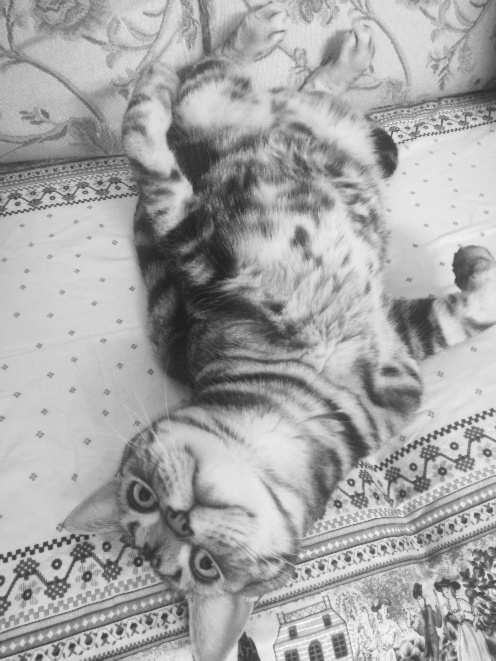
\includegraphics[width=0.3\textwidth,]{./img/cat_Guassian.jpg}}
        \subfigure[梯度滤波]{
            \label{Fig.Sfilt}
            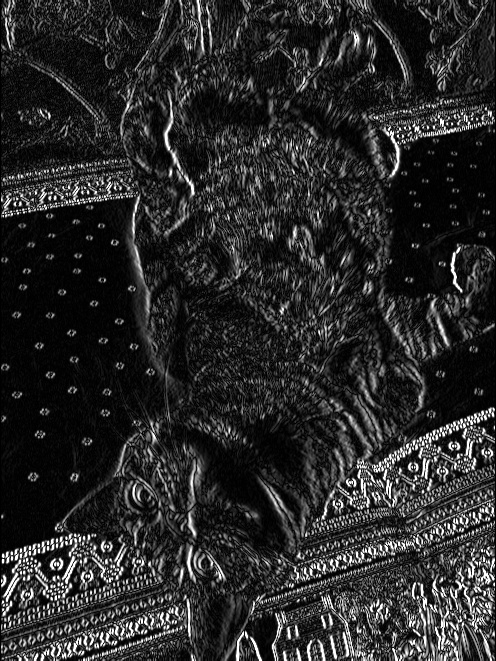
\includegraphics[width=0.3\textwidth]{./img/cat_Sobel.jpg}}
        \caption{基于梯度滤波的边缘检测}
        \label{Fig.filt}
    \end{figure}
\end{frame}

\begin{frame}{表格}
    \begin{table}[H]
        \centering
        \caption{顶层模块端口定义}
        \label{Tab.portTop}
        \begin{tabular}{|c|c|c|}
            \hline
            \multirow{3}*{输入端口} & clk0 & 时钟 \\ \cline{2-3}
            & ena0 & 使能 \\ \cline{2-3}
            & rst0 & 清零 \\ \hline
            \multirow{2}*{输出端口} & led & 显示 \\ \cline{2-3}
            & cout0 & 进位标志 \\ \hline
        \end{tabular}
    \end{table}
\end{frame}

\section{分栏}
\begin{frame}{分栏}
    \begin{columns}[c] % c-centering
        \column{0.5\textwidth} % Left part: figures
        \begin{figure} [H] % [H] is optional for current position
            \centering
            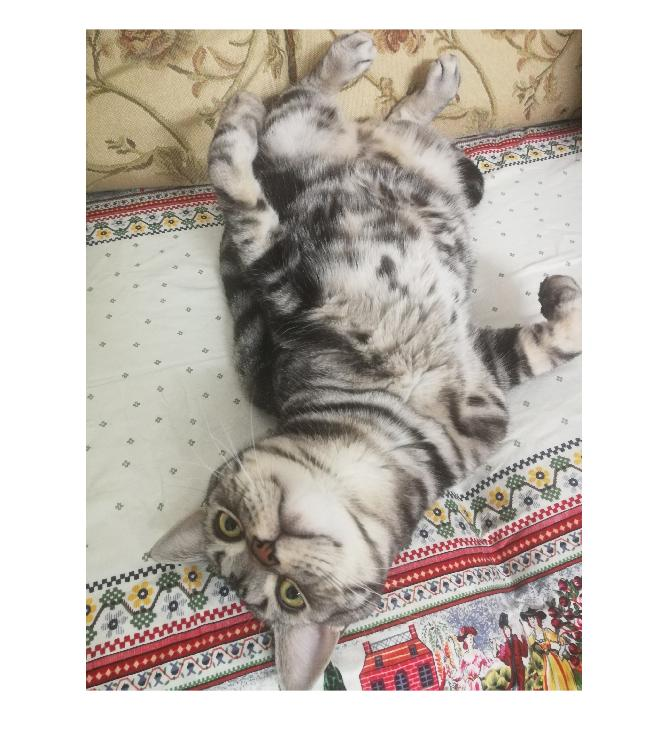
\includegraphics[width=0.7\textwidth]{./img/cat.jpg}
            \caption{可爱的小猫咪}
            \label{Fig.cat}
        \end{figure}
        \column{0.4\textwidth} % Right part: discriptions
        \begin{block}{文字说明1}
            这是一只小猫咪。
        \end{block}
        \begin{block}{文字说明2}
            这是一只美短。
        \end{block}
    \end{columns}
\end{frame}

%-------------------------------------------------------------%

%------------------------References---------------------------%
\section{参考文献}
\begin{frame}{参考文献}
    \bibliography{./reference.bib}
\end{frame}
%-------------------------------------------------------------%

%-----------------------Thanks Page---------------------------%
\begin{frame}{Thanks for listening}
    \begin{center}
        {\LARGE 谢谢!}
    \end{center}
\end{frame}
%-------------------------------------------------------------%

\end{document}